\subsection{风险监控失效}\label{sec:4}
\begin{frame}{巴塞尔II协议下系统性风险累积}
    在混业经营的大背景下,大型银行可利用在风险计量模型和内部信息方面的不对称性进行监管资本套利
    \begin{figure}[H]
        \includegraphics[width=0.8\linewidth]{img/basel.png}
        \caption{巴II对于系统性风险重视程度不足,结果导致系统性风险的大量累积}
    \end{figure}
\end{frame}

\begin{frame}{金融机构风控受制于竞争与贪婪}
    2006-07年各评级机构在竞争压力下失语,投行为了赚取更多佣金打包CDS为CDO,进一步吹大房贷市场的泡沫。
    \begin{figure}[H]
        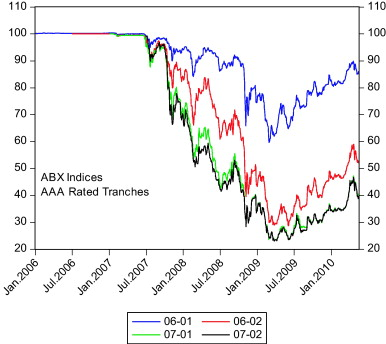
\includegraphics[width=0.7\linewidth]{img/abx.jpg}
        % \caption{ABX指数的波动}
        % \label{fig:abx}
    \end{figure}
\end{frame}

\begin{frame}{衍生品缺乏监管}
    对于某些复杂衍生品,其风险属性可能会急剧变化。在一天开始时的最佳对冲可能最终加剧一天结束时的风险暴露。
\begin{figure}[H]
    \centering
    \begin{minipage}[t]{0.48\linewidth}
        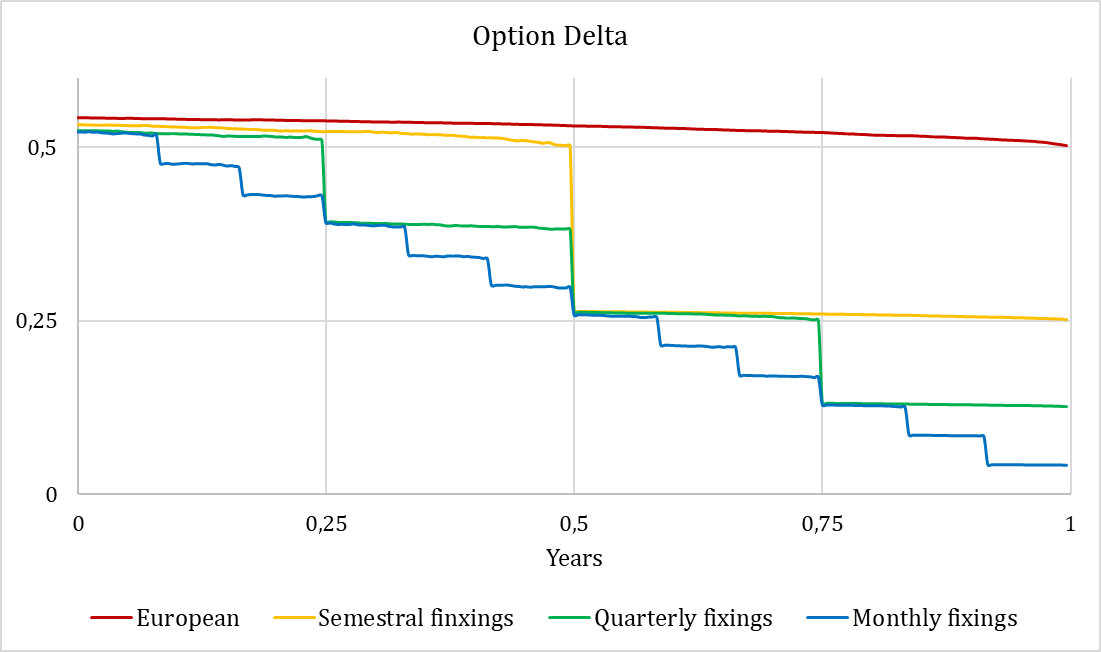
\includegraphics[width=\linewidth]{img/exo_delta.png}
    \end{minipage}
    \begin{minipage}[t]{0.48\linewidth}
        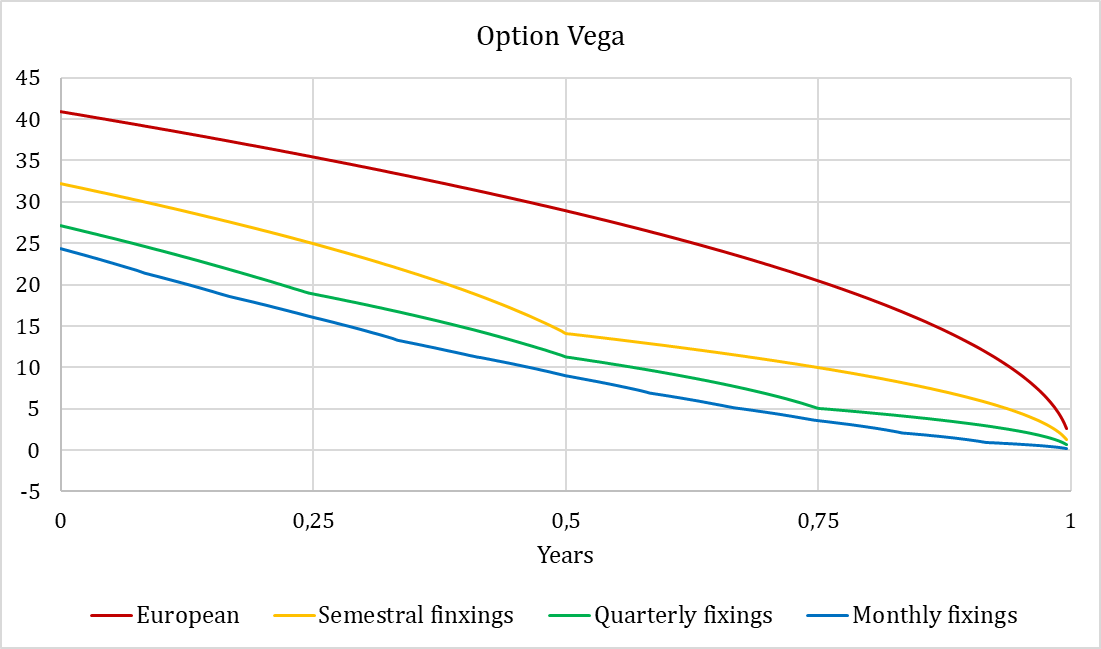
\includegraphics[width=\linewidth]{img/exo_vega.png}
    \end{minipage}
    \caption{亚式期权的$greexotics$}
    \label{fig:asia}
\end{figure}
\end{frame}

\subsection{风险管理措施失效}\label{sec:5}

\begin{frame}{管理措施受制于流动性}
    当市场上大量公司卖出时,流动性可能会被抽干,导致许多在平时可以使用的风险管理方案就无法再使用
    \begin{figure}[H]
        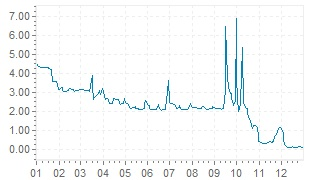
\includegraphics[width=0.6\linewidth]{img/libor2008.jpg}
        \caption{雷曼破产使各金融机构加紧与交易对手清算,市场流动性大幅降低}
        \label{fig:libor}
    \end{figure}
\end{frame}

\begin{frame}{公允价值计量加大对冲难度}
    对于大型组织来说,他们由于庞大的自身体量,参与到价格形成过程中时对价格影响非常大,使得他们做卖出决策时损失进一步放大。
    \begin{figure}[H]
        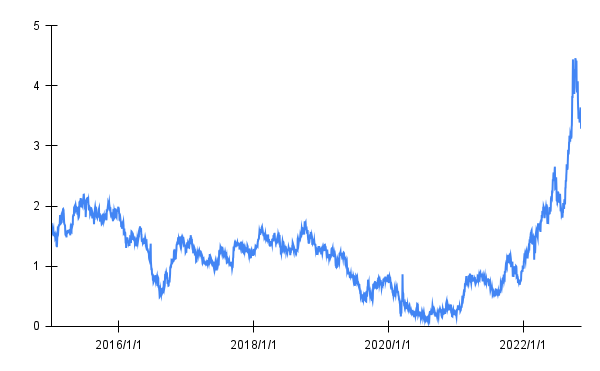
\includegraphics[width=0.6\linewidth]{img/british_bond.png}
        \caption{英国养老金平仓补交保证金导致进一步踩踏}
    \end{figure}
\end{frame}

\subsection{未使用适当的风险衡量标准}\label{sec:6}
\begin{frame}{VaR存在缺陷}
    短期VaR的衡量标准可能很低。VaR的缺陷包括:
\begin{enumerate}
    \item VaR不满足一致性
    \item 交易员可以在不违反VaR额度的前提下,构造一个较大风险的交易组合
    \item 资产价值不一定满足正态分布
    \item 交易组合价值变化在每天之间不一定相互独立
    \item 资产不一定可以被快速卖出或对冲
\end{enumerate}
解决方法是金融机构应该一方面考虑更长期的VaR,另一方面也要进行情景分析补充。
\end{frame}


\section{更全面的风险管理如何规避危机}
\begin{frame}
    金融危机暴露了彼时风险管理许多问题,但是并不意味着风险管理存在问题就一定会导致金融危机。
    
    我们也无法后验地判断通过全面风险管理成功规避了一次金融危机:阻止危机于危机形成之前也正是风险管理的价值所在。
    \begin{figure}
        \centering
        
\includegraphics[width=0.8\linewidth]{img/luna.drawio.png}
    \end{figure}
\end{frame}

\subsection{背景:LUNA归零、美联储加息}
\begin{frame}{大背景:美联储加息}
    全球热钱迅速减少,以比特币、以太坊为代表的加密货币交易量趋于平缓,其价格也开启了跌跌不休的模式。

\begin{figure}[H]
    \begin{minipage}[t]{0.48\linewidth}
        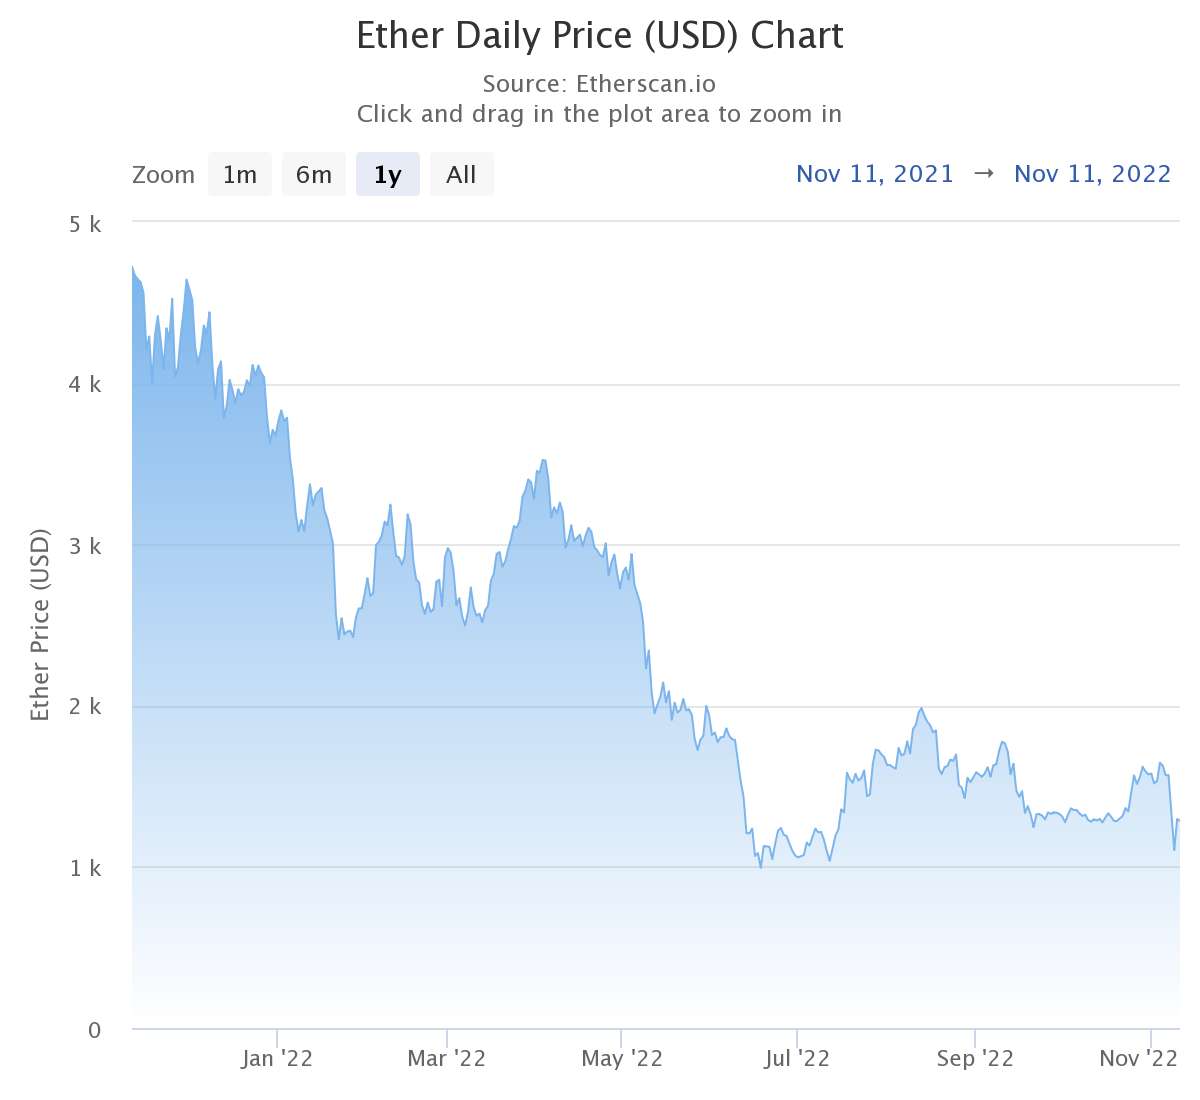
\includegraphics[width=\linewidth]{img/ether-daily-price-usd-ch.png}
        \caption{以太坊价格大幅回调}
    \end{minipage}
    \begin{minipage}[t]{0.48\linewidth}
        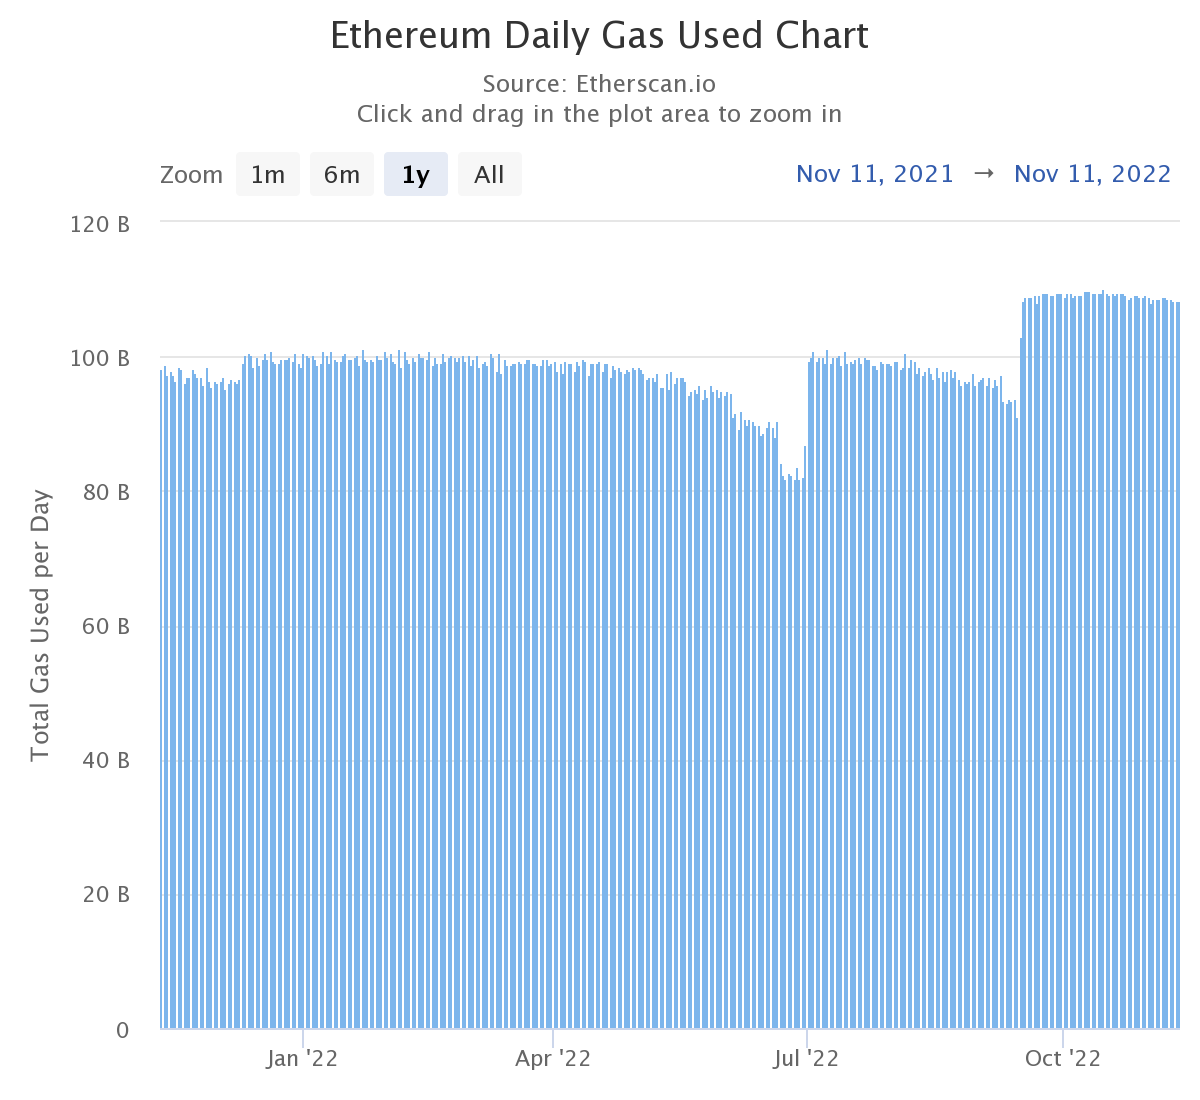
\includegraphics[width=\linewidth]{img/ethereum-daily-gas-used.png}
        \caption{以太坊交易量增长放缓}
    \end{minipage}
\end{figure}
\end{frame}

\begin{frame}{LUNA归零}
    \begin{figure}[H]
        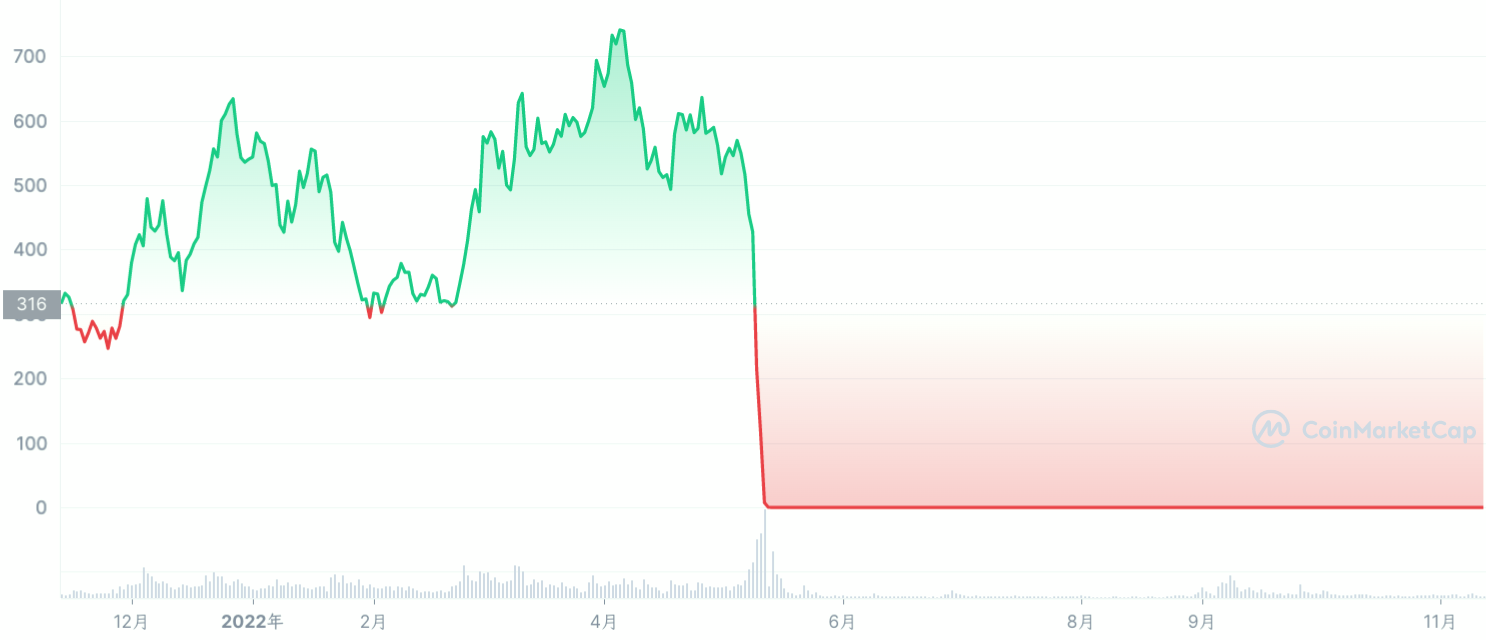
\includegraphics[width=0.6\linewidth]{img/luna.png}
        \caption{LUNA从120美元跌至0.00014美元,蒸发410亿美元}
    \end{figure}
    \only<1>{
        \begin{figure}[H]
            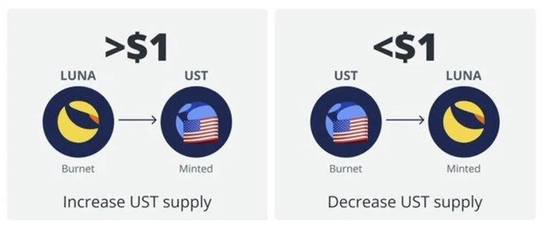
\includegraphics[width=0.6\linewidth]{img/ust.jpeg}
            % \caption{LUNA/UST的关系}
        \end{figure}
    }
    \only<2>{
        LUNA的暴跌带动加密货币全线大跌,压垮了多家风投机构,包括Voyager、Celsius、3AC等数家AUM数十亿美元的机构。加密货币两大交易所币安和FTX均尝试购买这些机构的剩余资产包,最终FTX在竞价中胜出。
    }
\end{frame}

\subsection{FTX的坠落:风险管理失败的例子}

\begin{frame}{FTX \& SBF}
    FTX由Sam Bankman-Fried(SBF)创立,在量化对冲基金中的经历使SBF信奉“在长期,风险爱好者和风险规避者都会输给风险中立者”。FTT 完全稀释市值为88.84亿美元
    
    FTX发行了FTT作为FTX的“股票”,以衍生品交易见长。在SBF高调成为美国民主党第二大捐助者后不久,FTT暴跌、FTX破产。
\begin{figure}[H]
    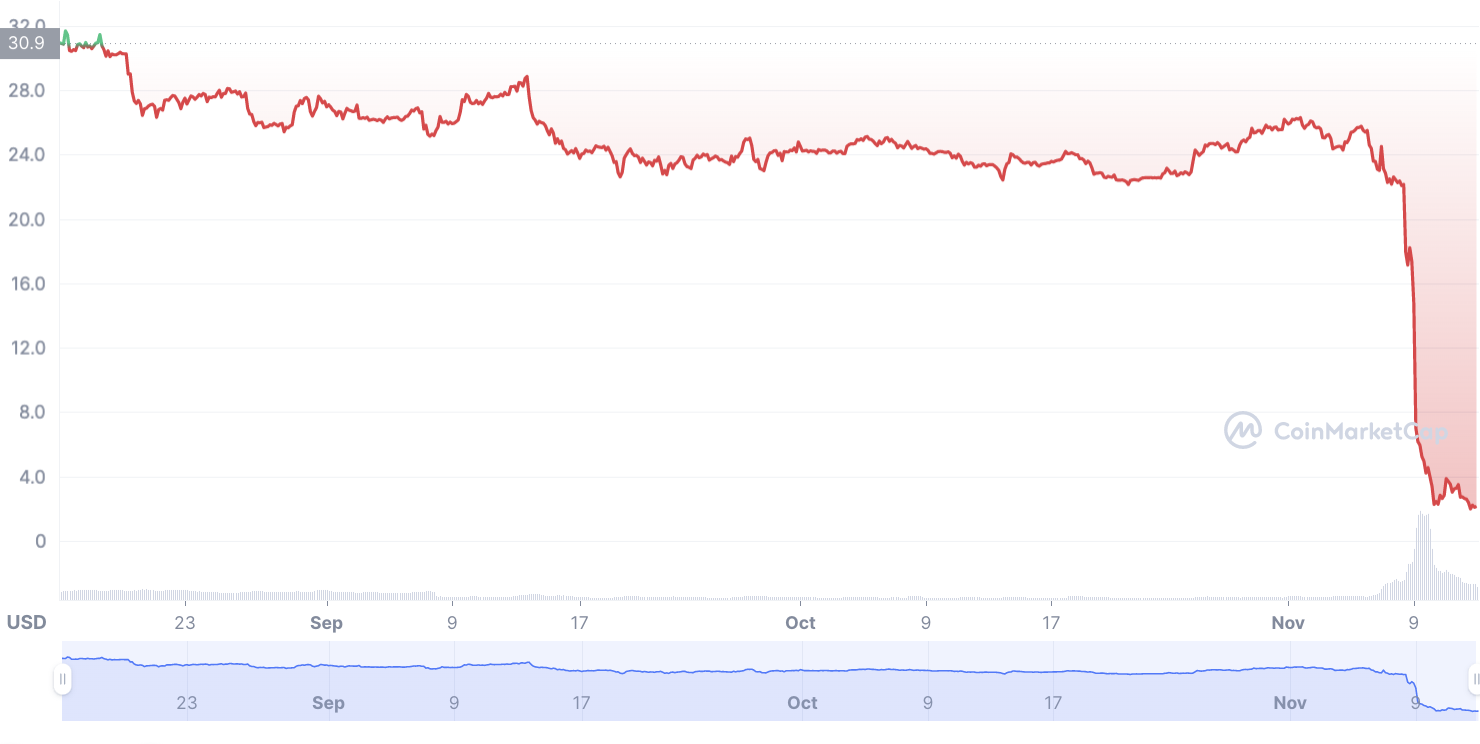
\includegraphics[width=0.7\linewidth]{img/ftt.png}
    \caption{FTT暴跌}
\end{figure}
\end{frame}

\begin{frame}
    \begin{table}[]
\caption{Alameda资产负债表}
\begin{tabular}{|llll|}
\hline
\multicolumn{2}{|c|}{资产(亿美元)}                            & \multicolumn{2}{c|}{负债及所有者权益(亿美元)} \\ \hline
\multicolumn{1}{|l|}{流通FTT}  & \multicolumn{1}{l|}{36.6} & \multicolumn{1}{l|}{非流通FTT} & 2.92 \\ \hline
\multicolumn{1}{|l|}{其他加密资产} & \multicolumn{1}{l|}{33.7} & \multicolumn{1}{l|}{贷款}     & 74   \\ \hline
\multicolumn{1}{|l|}{非流通FTT} & \multicolumn{1}{l|}{21.6} & \multicolumn{1}{l|}{其他}     & 3.08 \\ \hline
\multicolumn{1}{|l|}{非流通SOL} & \multicolumn{1}{l|}{9.04} & \multicolumn{1}{l|}{所有者权益}  & 66   \\ \hline
\multicolumn{1}{|l|}{流通SOL}  & \multicolumn{1}{l|}{2.92} &        &      \\ \hline
\multicolumn{1}{|l|}{股权投资}   & \multicolumn{1}{l|}{20}   &        &      \\ \hline
\multicolumn{1}{|l|}{现金及等价物} & \multicolumn{1}{l|}{1.34} &        &      \\ \hline
\multicolumn{1}{|l|}{其他}     & \multicolumn{1}{l|}{20.8} &        &      \\ \hline
\multicolumn{1}{|l|}{总计}     & \multicolumn{3}{c|}{146}                                       \\ \hline
\end{tabular}
\end{table}
    \only<1>{
        SBF的另一家公司Alameda Research为FTX上的做市商,提供流动性并赚取价差。
    }        
    \only<2>{\textbf{\nameref{sec:1}}:FTX和Alameda大肆收购了Voyager、Celsius等资产包,这些有毒资产消耗了大量的现金同时,也提高了FTX的杠杆率。而为了在加密寒冬中维持正常扩张、挑战币安地位,SBF暗中挪用了用户部分资金,迄今累计挪用接近100亿美元。}
    \only<3>{\textbf{\nameref{sec:2}}:SBF和Alameda以量化套利起家,其资金来源为在FTX套利过程中的资金沉淀,并以此进行短贷长投增厚收益。这种行为没有考虑到挤兑风险:在过去加密市场上行时,更多的用户进入市场使得这种行为可持续;而当加密寒冬到来时,用户提款可能会形成挤兑压倒FTX。}
    \only<4> {\textbf{\nameref{sec:3}}:Alameda资产负债表被曝光后,Alameda CEO曾表示愿以22美元的价格回购FTT,但面临5亿美元的缺口FTX管理层集体失联,导致市场信心进一步下挫,恐慌情绪蔓延。}
    \only<5>{\textbf{\nameref{sec:4}}:Alameda资产负债表两侧对于加密货币价格敏感程度差异巨大,没有对冲加密货币波动。Alameda利用FTT作为FTX的抵押品,从FTX借入其他资产,例如美元支持的稳定币。而在资产端为加密货币纯多头,在FTT价格波动较低时尚可平衡,而当整体加密货币向不利方向异常波动时容易资不抵债。}
    \only<6>{\textbf{\nameref{sec:5}}:Alameda资产中大部分为FTT,FTT完全稀释市值为88.84 亿美元,而FTX就持有超过50亿美元,考虑到流动性,若短时间大量抛售将难以维持最初估值。}
    \only<7> {\textbf{\nameref{sec:6}}:SBF信奉“风险中性者在长期期望上胜过风险爱好者和风险规避者”,FTX的风险衡量标准仅仅是“资产>负债”,在危机爆发初期SBF称其有能力支付用户存款。可当资产快速贬值时,该风险衡量标准缺陷暴露无疑,最终走向破产。}
\end{frame}


\subsection{风险管理如何规避危机}
\begin{frame}{币安何以坚挺}
    \begin{enumerate}
    \item \textbf{对已知风险的测量}:相较于FTX,币安对已知风险测量更为谨慎。币安同样表达过对Voyager等资产包的兴趣,在FTX暴雷初期也尝试并购FTX,但对资产包出价保持克制,对FTX并购前及时进行了\textbf{尽职调查},避免了LUNA的暴雷通过Voyager、FTX层层递进传导到自身。
    \item \textbf{对风险的考虑}:币安采取了储备金这一策略,即公布交易所现金资产的可验证证明,对挤兑风险更为重视。在FTX风波后,这一做法也在全行业逐步铺开。
    \item \textbf{对风险的沟通}:币安呈现相对扁平化管理,组织架构比较简单,没有Alameda这种身兼裁判员和运动员的实体,相较于FTX风险沟通更为顺畅。
    \end{enumerate}
\end{frame}
\begin{frame}{币安何以坚挺}
    \textbf{风险监控}:在FTX资产负债表暴露后,币安是最早清仓所持有FTT的玩家之一,损失相对较小。其他机构大多将FTX处投资减记至0美元
    \begin{table}[H]
        \centering
        \caption{FTX处投资减记至0美元的部分机构}
        \begin{tabular}{|c|c|c|}
            \hline
            机构&持仓最高峰值&投资金额\\\hline
            红杉资本&3.5亿美元&2亿美元\\
            淡马锡&3.2亿美元&3.2 亿美元\\
            Paradigm&3.15亿美元&2.15亿美元\\
            安大略教师养老金计划&1.25 亿美元&8000万美元\\\hline
        \end{tabular}
    \end{table}
\end{frame}
\begin{frame}{币安何以坚挺}
    \textbf{风险对冲措施}:币安也发行了自己的代币BNB,但明确表示过“切勿以自行创建的代币作为抵押品”,从源头上规避掉了FTX利用FTT空手套白狼的问题,BNB价格也是近期少有的上涨的主流加密货币。
    \begin{figure}[H]
        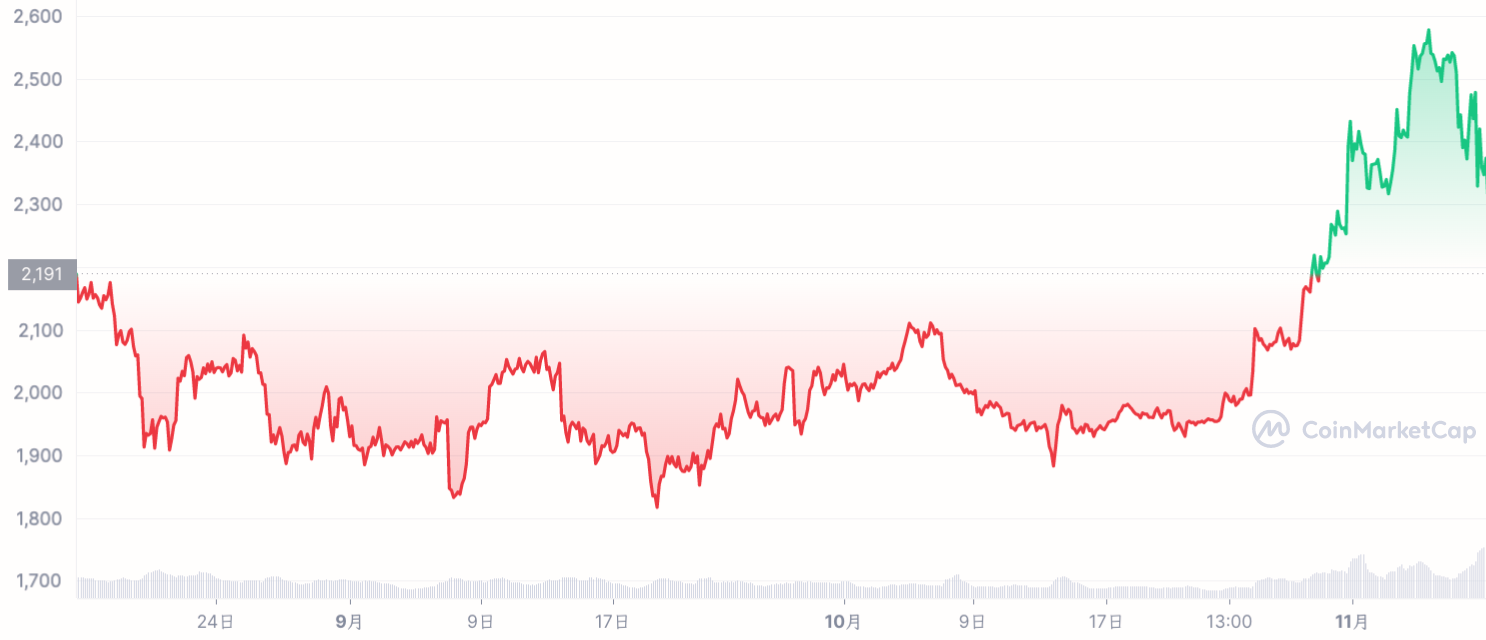
\includegraphics[width=\linewidth]{img/bnb.png}
        \caption{BNB代币价格}
    \end{figure}
\end{frame}

\begin{frame}{币安何以坚挺}
    \textbf{风险衡量标准}:币安的风险衡量标准更加保守。币安由于倡导去中心化的金融交易被各国监管所不容,因而其在处理金融问题中更为小心谨慎,以免吸引更多的火力。因而其自称不会追求“有效地使用资本”,需要有大量储备以防不时之需。
    \begin{block}{结论}
        从币安和FTX两家交易所的对比,我们可以看到,更加完备更加全面的风险管理可以避免危机的进一步传导与扩大,风险管理对危机的规避和处理是有价值的。
    \end{block}
\end{frame}


\section{结论}
\begin{frame}{金融危机$\ne$风险管理失败}
我们认为金融危机是不全面的风险管理的失败。金融危机产生于不全面的风险管理问题的集中爆发,例如对信贷市场的错误估计、衍生品的监管、金融机构的监管套利、流动性风险的长期忽视等等。风险管理也在金融危机中学习教训进一步补完,在经过金融危机历练后风险管理也在进一步地改善,如更为完善的监管体系、对流动性风险由定性转化为定量要求等,风险管理仍是有价值有意义的。
\end{frame}
